\section*{BreakthroughPP}
\newcommand{\myAlph}[1]{\char\numexpr`A-1+#1\relax}
\newcommand{\myalph}[1]{\char\numexpr`a-1+#1\relax}

\subsection*{Allgemein}
Die Breakthrough-Variante des Allgemeinen Programmierpraktikums (BreakthroughPP) ist ein Spiel für zwei Spieler, wobei ein Spieler mit roten und der andere mit blauen Steinen spielt.

BreakthroughPP wird auf einem Spielfeld mit quadratischen Feldern gespielt, die in $m$ Zeilen, gekennzeichnet mit aufsteigenden Nummern beginnend bei $1$, und $n$ Spalten, gekennzeichnet mit aufsteigenden Buchstaben beginnend bei $A$, angeordnet sind. Die untere linke Ecke des Spielfelds ist mit $A1$ gekennzeichnet.

\underline{Beispiel}

BreaktroughPP-Spielfeld aus $8 \times 8$ Quadraten.
\begin{center}
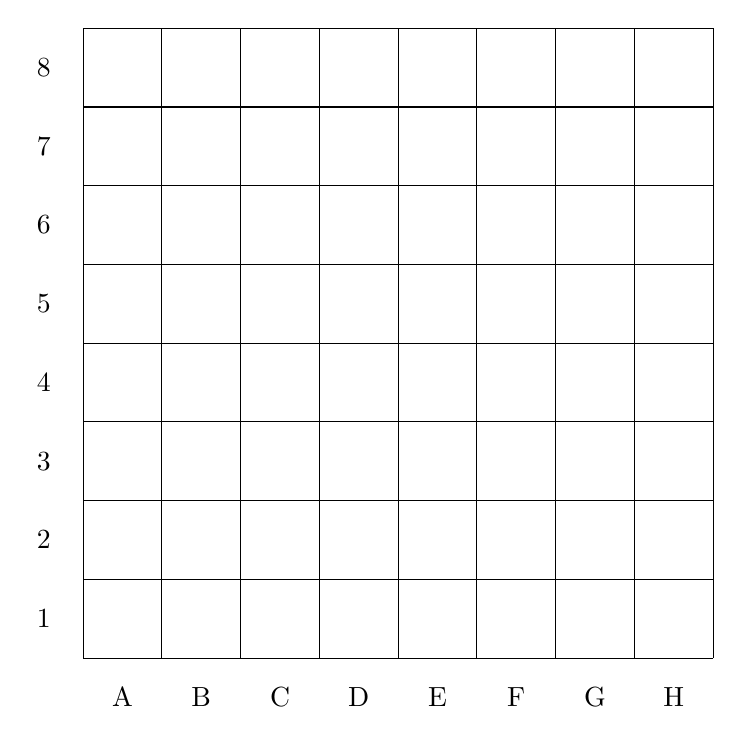
\begin{tikzpicture}
	\foreach \i in {0, ..., 8} {
		\draw [thin, black] (\i,0) -- (\i,8);
	}
	\foreach \i in {0, ..., 8} {
		\draw [thin, black] (0,\i) -- (8,\i);
	}
	\foreach \l in {1, ..., 8} {
		\draw node at (\l-0.5, -0.5) {\myAlph\l};
	}
	\foreach \n in {1, ..., 8} {
		\draw node at (-0.5, \n-0.5) {\n};
	}
\end{tikzpicture}
\end{center}

\subsection*{Startaufstellung}
Für $m, n$ gelten $6 \le m \le 26$ und $2 \le n \le 26$ und es gibt eine natürliche Zahl $k$ sodass \[k = \left\lfloor \frac{m + 3}{4} \right\rfloor \] 
Die unteren $k$ Zeilen von $1$ bis $k$ sind mit roten und die oberen $k$ Zeilen von $m-k+1$ bis $m$  mit blauen Steinen aufgefüllt.

Die Zeile $1$ wird hierbei als Startlinie des roten Spielers und die Zeile $m$ als Startlinie des blauen Spielers festgelegt.

\newpage
\underline{Beispiel}

Spielfelder mit $8 \times 8$, $6 \times 10$ und $14 \times 14$ Quadraten in Startaufstellung.
\begin{center}
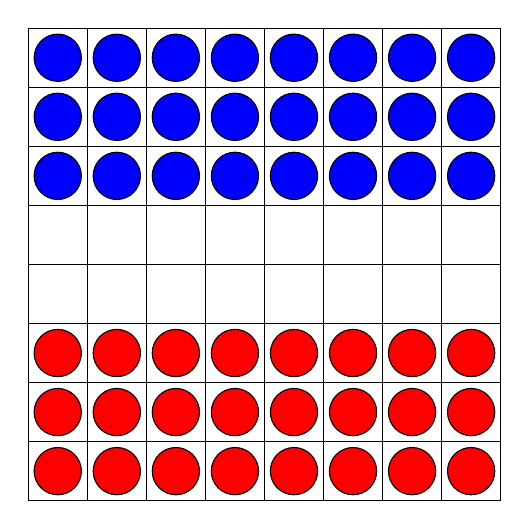
\begin{tikzpicture}[scale=0.75]
	% Cols
	\foreach \i in {0, ..., 8} {
		\draw [thin, black] (\i,0) -- (\i,8);
	}
	% Rows
	\foreach \i in {0, ..., 8} {
		\draw [thin, black] (0,\i) -- (8,\i);
	}
	% Red
	\foreach \r in {1, ..., 3} {
		\foreach \l in {1, ..., 8} {
			\draw [color=black, fill=red] (\l-0.5,\r-0.5) circle (0.4); 		
		}
	}
	% Blue
	\foreach \r in {6, ..., 8} {
		\foreach \l in {1, ..., 8} {
			\draw [color=black, fill=blue] (\l-0.5,\r-0.5) circle (0.4); 		
		}
	}
\end{tikzpicture} \hfill 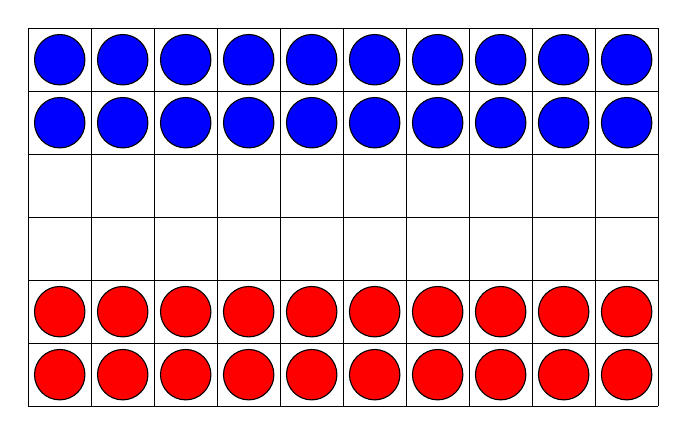
\begin{tikzpicture}[scale=0.8]
	% Cols
	\foreach \i in {0, ..., 10} {
		\draw [thin, black] (\i,0) -- (\i,6);
	}
	% Rows
	\foreach \i in {0, ..., 6} {
		\draw [thin, black] (0,\i) -- (10,\i);
	}
	% Red
	\foreach \r in {1, ..., 2} {
		\foreach \l in {1, ..., 10} {
			\draw [color=black, fill=red] (\l-0.5,\r-0.5) circle (0.4); 		
		}
	}
	% Blue
	\foreach \r in {5, ..., 6} {
		\foreach \l in {1, ..., 10} {
			\draw [color=black, fill=blue] (\l-0.5,\r-0.5) circle (0.4); 		
		}
	}
\end{tikzpicture}
\end{center}
\begin{center}
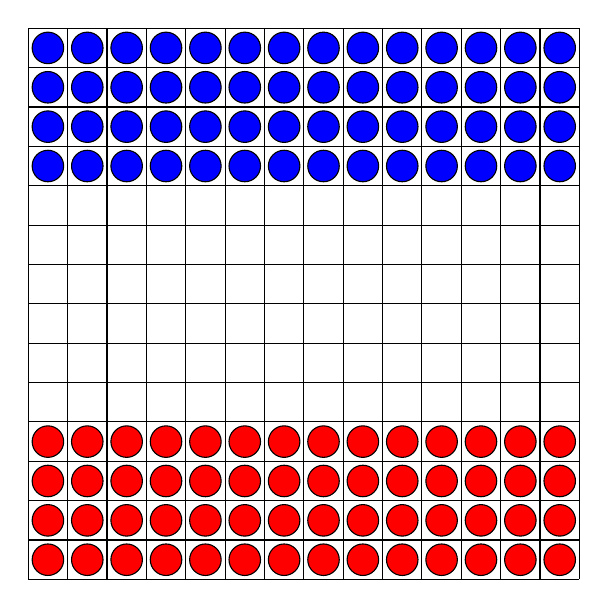
\begin{tikzpicture}[scale=0.5]
	% Cols
	\foreach \i in {0, ..., 14} {
		\draw [thin, black] (\i,0) -- (\i,14);
	}
	% Rows
	\foreach \i in {0, ..., 14} {
		\draw [thin, black] (0,\i) -- (14,\i);
	}
	% Red
	\foreach \r in {1, ..., 4} {
		\foreach \l in {1, ..., 14} {
			\draw [color=black, fill=red] (\l-0.5,\r-0.5) circle (0.4); 		
		}
	}
	% Blue
	\foreach \r in {11, ..., 14} {
		\foreach \l in {1, ..., 14} {
			\draw [color=black, fill=blue] (\l-0.5,\r-0.5) circle (0.4); 		
		}
	}
\end{tikzpicture}
\end{center}

\subsection*{Spielablauf}
Der Spieler mit den roten Steinen hat den ersten Zug. Dann wird abwechselnd gezogen, einen Zug auszulassen ist nicht möglich.
\medskip

\underline{Ziehen}

Alle Steine können sowohl vertikal als auch diagonal ein Feld in Richtung der gegnerischen Startlinie auf ein freies Feld ziehen. Springen ist nicht möglich.
\medskip

\underline{Schlagen}

Ein Stein kann einen gegnerischen Stein schlagen, indem er diagonal auf ein Feld mit einem gegnerischen Stein zieht. Der gegnerische Stein wird dann vom Brett genommen. Vertikales Schlagen ist nicht möglich.
\newpage

\underline{Beispiel}

\begin{center}
\begin{tikzpicture}[scale=1]
	% Grid
	\foreach \x/\y in {2/1,3/1,4/1,1/2,2/2,3/2,4/2,5/2,1/3,2/3,3/3,4/3,5/3,1/4,2/4,3/4,4/4,5/4,2/5,3/5,4/5} {
		\draw [thin, black] (\x-0.5,\y-0.5) -- (\x+0.5,\y-0.5); 
		\draw [thin, black] (\x+0.5,\y-0.5) -- (\x+0.5,\y+0.5); 
		\draw [thin, black] (\x+0.5,\y+0.5) -- (\x-0.5,\y+0.5); 
		\draw [thin, black] (\x-0.5,\y+0.5) -- (\x-0.5,\y-0.5); 
	}
	% Arrows
	\draw [draw=black,solid,line width=0.1em,-triangle 90,fill=black] (2,2) -- (1,3);
	\draw [draw=black,solid,line width=0.1em,-triangle 90,fill=black] (2,2) -- (2,3);
	\draw [draw=black,solid,line width=0.1em,-triangle 90,fill=black] (2,2) -- (3,3);
	
	\draw [draw=black,solid,line width=0.1em,-triangle 90,fill=black] (4,4) -- (3,3);
	\draw [draw=black,solid,line width=0.1em,-triangle 90,fill=black] (4,4) -- (4,3);
	\draw [draw=black,solid,line width=0.1em,-triangle 90,fill=black] (4,4) -- (5,3);
	
	% Red
	\foreach \x/\y in {2/2} {
		\draw [color=black, fill=red] (\x,\y) circle (0.4); 
	}
	% Blue
	\foreach \x/\y in {4/4} {
		\draw [color=black, fill=blue] (\x,\y) circle (0.4); 
	}
	
	% Label
	\draw (3, 0) node {\large{a})};
\end{tikzpicture} \hfill \begin{tikzpicture}[scale=1]
	% Grid
	\foreach \x/\y in {2/1,1/2,2/2,3/2,1/3,2/3,3/3,1/4,2/4,3/4,2/5} {
		\draw [thin, black] (\x-0.5,\y-0.5) -- (\x+0.5,\y-0.5); 
		\draw [thin, black] (\x+0.5,\y-0.5) -- (\x+0.5,\y+0.5); 
		\draw [thin, black] (\x+0.5,\y+0.5) -- (\x-0.5,\y+0.5); 
		\draw [thin, black] (\x-0.5,\y+0.5) -- (\x-0.5,\y-0.5); 
	}
	% Arrows
	\draw [draw=black,solid,line width=0.1em,-triangle 90,fill=black] (2,2) -- (1,3);;
	\draw [draw=black,solid,line width=0.1em,-triangle 90,fill=black] (2,2) -- (3,3);
	
	% Red
	\foreach \x/\y in {2/2} {
		\draw [color=black, fill=red] (\x,\y) circle (0.4); 
	}
	% Blue
	\foreach \x/\y in {2/3} {
		\draw [color=black, fill=blue] (\x,\y) circle (0.4); 
	}
	
	% Label
	\draw (2, 0) node {\large{b})};
\end{tikzpicture} \hfill \begin{tikzpicture}[scale=1]
	% Grid
	\foreach \x/\y in {2/1,3/1,4/1,5/1,1/2,2/2,3/2,4/2,5/2,6/2,1/3,2/3,3/3,4/3,
	5/3,6/3,1/4,2/4,3/4,4/4,5/4,6/4,2/5,3/5,4/5,5/5} {
		\draw [thin, black] (\x-0.5,\y-0.5) -- (\x+0.5,\y-0.5); 
		\draw [thin, black] (\x+0.5,\y-0.5) -- (\x+0.5,\y+0.5); 
		\draw [thin, black] (\x+0.5,\y+0.5) -- (\x-0.5,\y+0.5); 
		\draw [thin, black] (\x-0.5,\y+0.5) -- (\x-0.5,\y-0.5); 
	}
	% Blue
	\foreach \x/\y in {2/3,3/3,5/3} {
		\draw [color=black, fill=blue] (\x,\y) circle (0.4); 
	}
	% Arrows
	\draw [draw=black,solid,line width=0.1em,-triangle 90,fill=black] (2,2) -- (1,3);
	\draw [draw=black,solid,line width=0.1em,-triangle 90,fill=black] (2,2) -- (3,3);
	\draw [draw=black,solid,line width=0.1em,-triangle 90,fill=black] (5,2) -- (4,3);
	
	% Red
	\foreach \x/\y in {2/2,5/2,6/3} {
		\draw [color=black, fill=red] (\x,\y) circle (0.4); 
	}
	
	% Label
	\draw (3.5, 0) node {\large{c})};
\end{tikzpicture}
\end{center}
\begin{enumerate}[label=\alph*)]
\item Der rote und blaue Spieler haben je drei Möglichkeiten zum Zug.
\item Der rote Spieler kann nur diagonal ziehen.
\item Der linke rote Stein kann sowohl nach links oben ziehen als auch nach rechts oben schlagen. Der rechte rote Stein kann nur nach links oben ziehen, da ein eigener Stein nicht geschlagen werden kann.
\end{enumerate}

\subsection*{Ende des Spiels}
Das Spiel ist gewonnen, wenn ein Stein die Ziellinie des gegnerischen Spielers erreicht. Ob in diesem Zug normal gezogen oder geschlagen wurde ist hierbei irrelevant.

Da in jedem Zug ein Stein bewegt werden muss und sich aufgrund der Möglichkeit diagonal zu ziehen und zu schlagen nicht alle Steine beider Spieler gegenseitig blockieren können, kann das Spiel nicht unentschieden enden.

\subsection*{Einfache Strategie}
\dots